Natevení filtru typu DP pro \(f_{m} =  \qty{10}{\micro Hz}\) :
\begin{align*}
    \tau &= \frac{1}{\omega} \\
    R\cdot C &= \frac{1}{2\cdot \pi \cdot f_{RC} } \\
    R\cdot C &= \frac{1}{2\cdot \pi \cdot \num{10e-6} } \\
    R\cdot C &= \num{16e3} \\
\end{align*}

Pokud zvolíme \(R=\qty{100}{M\ohm}\), pro kondenzátor vychází \(C=\num{16e3}/\num{100e6} = \qty{160}{\micro F}\) 

\begin{figure}[h!]
    \centering
    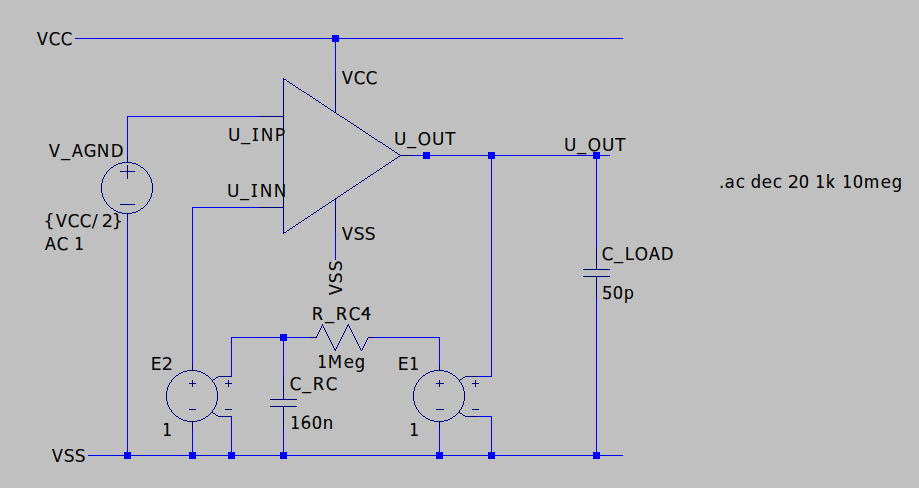
\includegraphics[scale=0.5]{spiceAC.png}
    \caption{Zapojení pro .AC analýzu.}
    \label{fig:spiceAC.png}
\end{figure}

\begin{figure}[h!]
    \centering
    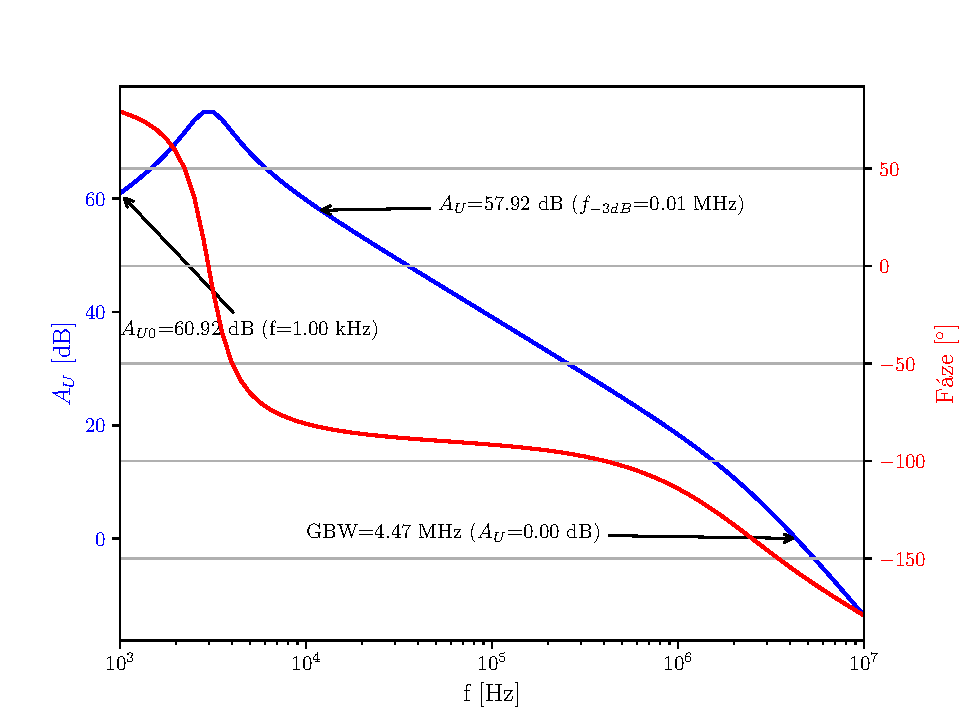
\includegraphics[]{AC.pdf}
    \caption{Výsledky .AC analýzy.}
    \label{fig:AC.pdf}
\end{figure}


